\documentclass[letterpaper,10pt]{book}

\usepackage[T1]{fontenc}
\usepackage[latin1]{inputenc}
\usepackage{geometry}
\usepackage{graphics,color}
\geometry{letterpaper}
\usepackage{array}
\usepackage{floatflt}
\usepackage{subfloat}
\usepackage{lineno}
\usepackage{amsmath}
\usepackage{fancyvrb}
%\usepackage[listofnumwidth=5.5em]{subfig}
\usepackage{tocloft}
\usepackage{longtable}

%  for showing script lines as they appear in GMAT
\usepackage{verbatim}


\oddsidemargin  0.0in \evensidemargin 0.0in \textwidth      6.5in
\headheight     0.25in \topmargin      0.0in \textheight=8.5in


% More space for figure numbers
\setlength{\cftfignumwidth}{3em}
% Space between elements of the list
%\setlength{\cftbeforefigskip}{0.1cm}
% Space before chapter entries in the TOC
%\setlength{\cftbeforechapskip}{0.2cm}
% Space before parts in the TOC
%\setlength{\cftbeforepartskip}{0.7cm}

%\setlength{\emergencystretch}{6em}
%\pretolerance=10000
%\tolerance=10000

%\define@key{caption}{listofnumwidth}[4em]{\def\sf@numwidth{#1}}
\begin{document}

%----------------------------------------------------------
%----------------Cover Page Stuff -------------------------
%----------------------------------------------------------
\thispagestyle{empty}
\begin{center}
{\renewcommand{\thefootnote}{\fnsymbol{footnote}} { \Huge \bf
General Mission Analysis Tool\\ (GMAT)\\ Graphical User Interface
Test Plan }}
\end{center}
\begin{center}
{\renewcommand{\thefootnote}{\fnsymbol{footnote}} { \Huge \bf
 DRAFT }}
\end{center}

\vspace{1.0 in}

\begin{figure}[ht]
\begin{center}

\includegraphics[421,303]{Images/GMATSplash.png}
\end{center}
\end{figure}
%
%\vspace{0.25 in}
\begin{center}
\Large{NASA Goddard Space Flight Center\\
Greenbelt RD\\
Greenbelt, MD 20771}
\end{center}

\clearpage\clearpage

\verbatiminput{ImpulsiveBurnPanel.txt }

\end{document}
%----------------------------------------------------------
%----------------  The document body-----------------------
%----------------------------------------------------------
\tableofcontents \clearpage \listoffigures \clearpage

\chapter{General Tests}

\section{Main Window and Menu Bar}

\section{Tests That Apply to All Panels and Dialogue Boxes}
\label{Sec:GeneralTests}


%  This is the list of tests associated with panel aesthetics
\noindent\textbf{Aesthetics}\\

\noindent Description:  This set of tests is to verify look and feel
of a panel.

%
\begin{itemize}
    \item Can all of the data input fields be seen at the default panel
    size for all tabs on panel?  This includes bounding boxes.
    %
    \item Is there too much blank space surrounding the data area?
    %
    \item Is there too little blank space surrounding the data area?
    %
    \item Can the window be resized so that the data cannot be seen?
    %
\end{itemize}
\vspace{.25 in}

%
\noindent\textbf{General Panel Functionality}\\

\noindent Description:  This is the list of tests associated with
basic  panel functionality: open, close, rename, minimize, ok,
cancel, help, show script, command summary.

\begin{itemize}
    %
    \item From the appropriate tree (Resource or Mission), can you create a new object of the type being tested?
    %
    \item Can you double left click and open the panel of the new
    object?
    %
    \item Can you rename the new object?
    %
    \item If there is a default object of the type being tested, can you rename
    it?  Check at least one place in the mission sequence or resource tree to
    ensure the new name is being used.
    %
    \item Can you make a minor change on the panel, hit ok, and then rename the object?
    %
    \item Can you make a minor change on the panel, hit ok, reopen,
    and see that the change was saved?
    %
    \item Can you make a minor change on the panel, hit apply, then
    hit show script to see that the apply button saved the change
    and  it is visible in the script?
    %
    \item Can you open the panel, and while the panel is open,
    change the name in the resource tree.  Check at least one place in the mission sequence or resource tree to
    ensure the new name is being used.
    %
    \item Can you open the panel and hit cancel and the panel
    closes?
    %
    \item Can you open the panel, make a minor change in the data,
    hit cancel, reopen the panel and confirm the data was not saved?
    %
    \item Can you open the panel and
    click the small ``x" button in the upper right hand corner and close the panel?
    %
    \item Can you open the panel, make a minor change in the panel,
    click the small x button in the upper left hand corner, and be
    prompted to save data before closing?
    %
    \item When you click the minimize icon does the panel minimize?
    %
    \item When the panel is minimized, can you hit the maximize icon
     and the panel reopens to previous size?
    %
    \item When the panel is open and you use the tab key to
    negotiate panel, does the action agree with style and GUI
    philosophy?
\end{itemize}
\vspace{.25 in}

%
\noindent\textbf{Panel Data Element Completeness and Correctness}\\

\noindent Description: This set of tests verifies that all data
elements that should appear on the panel indeed appear on the panel.
It also tests that all elements that should appear in show script
appear there and that items that should not appear in show script do
not appear there.

\begin{itemize}
    %
    \item Verify that only data elements that occur in the Range
    Test Plan appear in show script and that the user does not see
    any other object fields.   Also check that defaults agree with
    Range Test Plan.
    %
    \item Verify that all elements that should appear in show script
    appear.  (See range test plan)
    %
    \item  Verify that all data elements
    that appear in Show Script also appear on the GUI.  This
    means that if you can set something in the script, ensure that it
    appears in the GUI.
    %
\end{itemize}
\vspace{.25 in}


\section{Tests for Specific Data Element Types on Panels}

 \begin{longtable}{p{1.25 in} |p{4.5 in} }
 \caption
 [Tests for Data Objects on All Panels]
 {Tests for Data Objects on All Panels \label{Table:DataElementTests}}\\
 \hline\hline
% \multicolumn{2}{@{*}c@{*}}%
%      {This part appears at the top of the table}\\
 Element Type & Tests\\
 \hline
 \endfirsthead
 \caption[]{(Tests for Data Objects on All Panels...continued)}\\
 \hline\hline
 Element Type & Tests\\
 \hline\hline
 \endhead
 \hline
 % This goes at the&bottom.\\
 \hline
 \endfoot
 \hline
 \hline
 \endlastfoot
%-----------------------------------------------------------------------
%-----------------------Begin Table Here--------------------------------
%-----------------------------------------------------------------------
% ---- Column 1--------%
Check Boxes &
% ---- Column 2--------%
\begin{itemize} \vspace{-.25 in}
\item Set all check boxes to off (unchecked), hit show script, and verify that the functionality is
indeed turned off for each radio button and check box.
%
\item Set all check buttons to on (checked), hit apply, and show script
and verify that the functionality is indeed turned on for each radio
button and check box.
\end{itemize} \\
\hline
% ---- Column 1--------%
Radio Buttons &
% ---- Column 2--------%
\begin{itemize} \vspace{-.25 in}
   \item For each radio button on panel, select the button, and ensure that it activates
   and all others are deactivated.  Hit Apply, and then check show
   script to ensure that the configuration was properly saved.
\end{itemize} \\
\hline
%-------------- This is the beginning of a new row!!!----------------------
% ---- Column 1--------%
Combo Boxes &
% ---- Column 2--------%
\begin{itemize} \vspace{-.25 in}
\item  For each combo box on the panel, ensure that all options that
appear in Range Test Plan appear in the pull down menu.
%
\item  For each Combo box on the panel, select each allowable option, hit apply and show script
and check to see that the option was correctly saved.
%
\item Check to ensure that the combo box is not editable.
\end{itemize} \\
\hline
%-------------- This is the beginning of a new row!!!----------------------
% ---- Column 1--------%
Text Fields &
% ---- Column 2--------%
\begin{itemize} \vspace{-.2 in}
\item For each text field enter ``DNE" and ensure that if GMAT should reject this string that the string is
rejected. ( Currently, this is not an acceptable value for any GMAT
field unless the user has created an appropriate object type and
named it DNE, and is using it correctly in the GUI. )
%
\item Perform all range tests as described in Range Test Plan.
%
\item For all numeric fields, enter an allowed numeric value, hit
apply and show script and check that the value was saved.
%
\item If user-defined objects can appear in the combo box, create
one object for all allowable object types for the particular combo
box, and ensure that it appears in the combo box.  Also, hit apply
and ensure that each case appears in show script.
%
\end{itemize} \\
\hline
%-------------- This is the beginning of a new row!!!----------------------
% ---- Column 1--------%
Action Buttons &
% ---- Column 2--------%
\begin{itemize} \vspace{-.2 in}
\item For each button ensure that clicking on the button brings up the appropriate panel.
\item For the panel opened up, perform all tests defined in Section \ref{Sec:GeneralTests} and Table \ref{Table:DataElementTests}
\end{itemize} \\
\hline
%-------------- This is the beginning of a new row!!!----------------------
% ---- Column 1--------%
Selection Lists &
% ---- Column 2--------%
\begin{itemize} \vspace{-.2 in}
\item First Item
\item Second Item
\end{itemize} \\
\hline

%-------------- This is the beginning of a new row!!!----------------------
% ---- Column 1--------%
Tabbed Panels &  % ---- Column 2--------%
\begin{itemize} \vspace{-.2 in}
\item First Item
\item Second Item
\end{itemize} \\
\end{longtable}


%% ---- Column 2--------%
%\begin{itemize} \vspace{-.2 in}
%\item First Item
%\item Second Item
%\end{itemize} \\
%\hline


\chapter{Specific Tests for Panels and Dialogue Boxes Under Resources Tree}

\section{Propagator Panel}

%------------------------------------------------------------
%--------------  Main Propagator Panel Image ----------------
%------------------------------------------------------------

\begin{figure}[ht]
\begin{center}
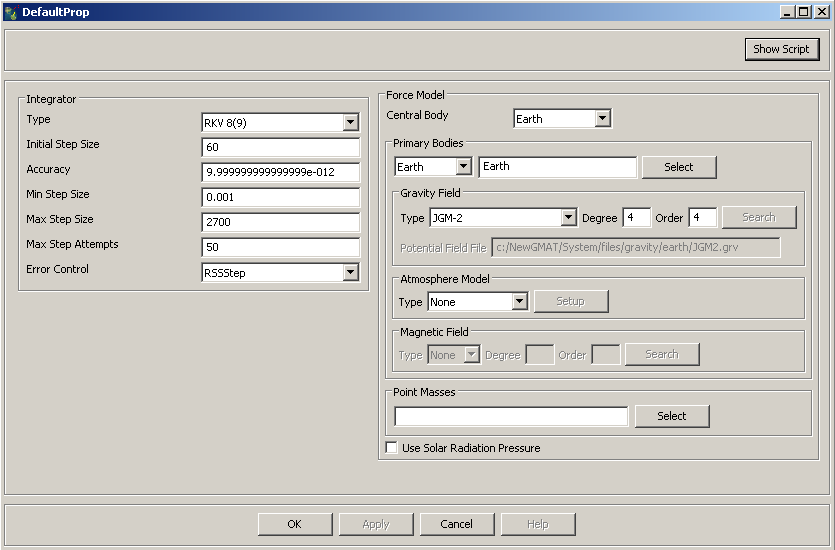
\includegraphics[468,337]{Images/Propagator.png}
\caption{\label{figure:Propagator} The Propagator Panel}
\end{center}
\end{figure}

%------------------------------------------------------------
%--------------  Main Propagator Panel Image ----------------
%------------------------------------------------------------


\textbf{Radio Buttons and Check Boxes}\\

\noindent For the radio buttons and check boxes listed below perform
the tests listed in Table \ref{Table:DataElementTests}:
%
\begin{itemize}
    %
    \item Use Solar Radiation Pressure
    %
\end{itemize}


\noindent\textbf{Combo Boxes}\\

\noindent For the combo boxes listed below perform the tests listed
in Table \ref{Table:DataElementTests}:
%
\begin{itemize}
    %
    \item Integrator/Type
    %
    \item Integrator/Error Control
    %
    \item ForceModel/Central Body
    %
    \item ForceModel/Primary Bodies
    %
    \item ForceModel/Gravity Field/Type
    %
    \item ForceModel/Atmosphere Model/Type
\end{itemize}


\noindent\textbf{Text Fields}\\

\noindent For the text fields listed below perform the tests listed
in Table \ref{Table:DataElementTests}:
%
\begin{itemize}
    %
    \item Integrator/Initial Step Size
    %
    \item Integrator/Accuracy
    %
    \item Integrator/Min Step Size
    %
    \item Integrator/Max Step Size
    %
    \item Integrator/Max Step Attempts
    %
    \item ForceModel/Gravity Field/Degree
    %
    \item ForceModel/Gravity Field/Order
    %
    \item AtmosphereModel/Setup/Solar Flux
    %
    \item AtmosphereModel/Setup/Average Solar Flux
    %
    \item AtmosphereModel/Setup/Geomagnetic Index
    %
    \item AtmosphereModel/FileName
    %
\end{itemize}

\noindent \emph{Select ABM under Integrator/Type to see these Text
Fields}
\begin{itemize}
    %
    \item Integrator/Nominal Integration Error
    %
    \item Integrator/Min Integration Error
    %
\end{itemize}


\noindent\textbf{Buttons}\\

\noindent For the Buttons listed below perform the tests listed in
Table \ref{Table:DataElementTests}:
%
\begin{itemize}
    %
    \item Force Model/Primary Bodies/ Select
    %
    \item Force Model/Atmoshere Model/Setup
    %
    \item Force Model/Point Masses/Select
    %
\end{itemize}



\noindent\textbf{Selection Lists}\\

There are no Selection Lists on the Propagator panel.\\



\noindent\textbf{Tabbed Panels}\\

There are no Tabbed Panels on the Propagator panel\\



\noindent\textbf{Numeric Tests}\\

There are no Numeric Tests for the Propagator panel.\\



\noindent\textbf{Panel Specific Field Coupling Tests}\\

These tests are related to interactions between different data
elements on the panel.\\

\begin{itemize}
    %
    \item Add Sun, Luna, Mercury, and Venus to Primary bodies list.  Now
    click on the Select button under point masses.  Ensure that all
    bodies that appear in the primary bodies list do not appear
    on the selection panel for point masses.
    %
    \item Create a new propagator.  Add Sun, Luna, Mercury, and Venus to point masses list.  Now
    click on the Select button under Primary Bodies.  Ensure that all
    bodies that appear in the point mass list do not appear
    on the selection panel for Primary Bodies.
    %
    \item Create a new propagator.  Add Sun, Luna, Mercury, and Venus to point masses
    list.  Click apply and hit show script and verify that the
    Sun, Luna, Mercury, and Venus appear in the list of
    point masses.
    %
    \item Create a new propagator.  Add Sun, Luna, Mercury, and Venus
    to Primary Bodies list.  Click apply and hit show script and verify that the
    Earth, Sun, Luna, Mercury, and Venus appear in the list of
    primary bodies.
    %
    \item Create a new propagator.  Add Luna, Mars and Venus as Primary Bodies. Now:

    \begin{itemize}
    %
    \item  In the combo for primary bodies select Luna.  Now in the
    Gravity Field/Type combo box, ensure only LP165 and Other appears in
    the options.  Ensure the Atmosphere/Type combo box is
    disabled.
    %
    \item  In the combo for primary bodies select Mars.  Now in the
    Gravity Field/Type combo box, ensure only Mars-50C and Other appears in
    the options. Ensure the Atmosphere/Type combo box is
    disabled.
    %
    \item  In the combo for primary bodies select Venus.  Now in the
    Gravity Field/Type combo box, ensure only MGNP-180U and Other appears in
    the options. Ensure the Atmosphere/Type combo box is
    disabled.
    %
    \item In the combo for primary bodies select Earth. Click the ForceModel/GravityField/Search button.  Select a
    valid gravity model for earth, that is different from the model already in the panel.  Hit
    ok. Verify that the new model is in the text box.  Hit apply and
    show script and verify that the new model is shown in the
    script.
    \end{itemize}

\end{itemize}


\chapter{Specific Tests for Panels and Dialogue Boxes Under Mission Tree}

\backmatter

\begin{thebibliography}{poseidon} % start the bibliography

\bibitem[Bazman]{Bazman} http://members.tripod.com/~bazman/checklist.html

\bibitem[Black]{Black} Rex Black, ``Managing the Testing Process,'' Second Edition, WileyPublishing, 2002.

\bibitem[Craig]{Craig} Rick D. Craig and Stefan P. Jaskiel, ``Systematic Software Testing,'' Artech House, 2002.

\bibitem[MTP]{MTP} GMAT Analysis Team, ``General Mission Analysis Tool (GMAT) Master Test Plan.''

\bibitem[GDT]{GDT} GMAT Development Team, ``General Mission Analysis Tool (GMAT) Architectural
Specification.''

\bibitem[hughes]{hughes} Steven P. Hughes, ``General Mission Analysis Tool (GMAT) Mathematical
Specification.''

\bibitem[hughes2]{hughes2} Steven P. Hughes, ``General Mission Analysis Tool (GMAT) User's Guide.''

\bibitem[Schiff]{schiff} Conrad Schiff, ``Personal Correspondence''

\bibitem[matlab]{MATLAB} The MathWorks, Inc, ``MATLAB'', available from http://www.mathworks.com.

\bibitem[OOo]{OOo} OpenOffice.org, ``OpenOffice'', available from http://www.openoffice.org/.

\end{thebibliography}

\end{document}
